\chapter{Stand der Technik}
\label{ch:StandDerTechnik}
In diesem Kapitel werden Begriffe und Konzepte eingeführt und erklärt, welche durch die Arbeit verwendet
werden. Somit kann diese Sektion als ein Nachschalgewerk genutzt werden um allfällige Lücken zu schliessen
und Zusammenhänge zwischen den einzelnen Konzepten besser zu verstehen.

\section{Technologische Grundlagen}
\label{sec:technische-grundlagen}
In diesem Abschnitt werden die wichtigsten technologischen Grundlagen für das Projekt behandelt. Diese Grundlagen
beinhalten vor allem Begriffdefinitionen, welche in den weiteren Kapiteln immer wieder verwendet werden. Die meisten
dieser Grundlagen sind Überbegriffe, welche vorausgesetzt werden um die detaillierten Konzepte in
\fullref{sec:technische-konzepte} zu verstehen.

\subsection{Natural Language Generation}
\label{sub:natural-language-generation}
Natural Language Generation (NLG) (\cite{wikipedia_2019_nlg}) (\textit{dt.} natürliche Textgenerierung), ist ein
Unterbereich von Artificial Intelligence, welcher sich auf die automatisierte Generierung von geschriebenem oder
gesprochenem Text fokussiert.
\newline
\newline
Das Ziel von \gls{NLG} ist es sequenzielle Daten zu generieren, welche nicht von menschlichen Sequenzen unterschieden
werden können. Diese Sätze sollen aussagekräftig und ausserdem grammatikalisch korrekt sein. Dies geschieht in einem
Bruchteil der Zeit welche ein Mensch dafür bräuchte.
\newline
\newline
Etabliert hat sich die Textgenerierung vor allem im Bereich des Journalismus, in denen Nachrichten auf Daten basieren.
So werden heutzutage zum Beispiel Nachrichtentexte für Wetter-, Sport und Finanzberichte zu einem grossen Teil von
NLG-Systemen generiert.

\subsection{Natural Language Processing}
\label{sub:natural-language-processing}
Natural Language Processing (NLP) (\cite{wikipedia_2019_nlp}) (\textit{dt.} natürliche Textverarbeitung) ist ein
Unterbereich von Artificial Intelligence, welcher sich auf die Verarbeitung von natürlicher Sprache fokussiert. Ziel ist
es, eine direkte Kommunikation auf Grund natürlicher Sprache, zwischen dem Menschen und dem Computer herzustellen. NLP
wird z.B. in Sprachassistenten wie Siri oder Alexa verwendet.

\subsection{Neural Style Transfer}
\label{sub:neural-style-transfer}
Der Bereich von \gls{NST} ist eine junge, erst 2015, von Gatys et al. (\cite{gatys2015neural}) eingeführte Technik,
welche sich auf die Manipulation von Bildern bezieht um das Aussehen oder den visuellen Stil eines anderen Bildes zu
übernehmen. \gls{NST} verwenden sehr tiefe Netze, um die Bildtransformation durchzuführen. Häufige Anwendungen für
\gls{NST} sind die Erstellung von künstlichen Kunstwerken aus Fotos, zum Beispiel durch die Übertragung des Aussehens
berühmter Gemälde auf Fotos. \gls{NST} findet die Anwendung vor allem in verschiedenen mobilen Apps.
\begin{figure}[H]
	\centering
	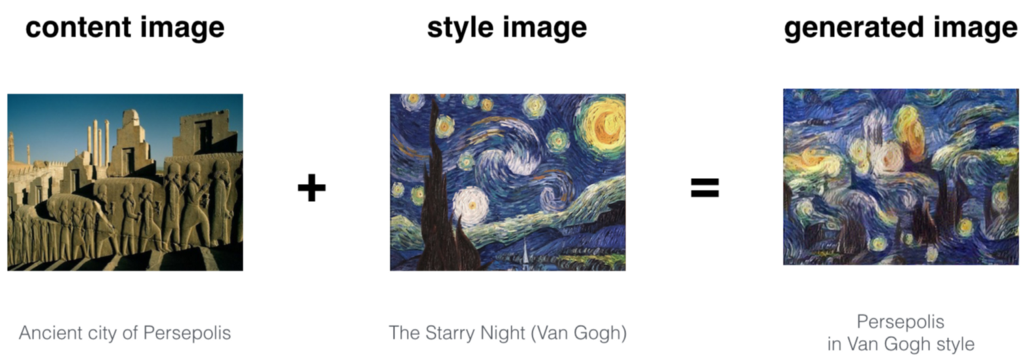
\includegraphics[scale=0.3]{neural_style_transfer}
	\caption{Neural Style Transfer für artistische Gemälde}
	\label{fig:neural-style-transfer}
\end{figure}
\noindent
Infolge des Erfolgs der Technik für artistische Gemälde wurde diese über die Jahre weiter verfolgt. Dabei wird ebenfalls
versucht die Technik auf andere Bereiche anzuwenden. So gibt es eine Bewegung (\cite{fuzhenxin_2019}), die versucht
\gls{NST} auch für Texte zu nutzen. 
\newline
\newline
Dabei werden in der Forschung momentan verschiende \gls{NST} untersucht. Beliebt sind dabei beispielsweise der Transfer
von \flqq positiv\frqq \ zu \flqq negativ\frqq, \flqq informell\frqq \ zu \flqq formell\frqq \ oder auch \flqq
aggressiv\frqq \ zu \flqq passiv\frqq. Dabei wurden in der untersuchten Literatur vorallem die Transfer \flqq
positiv\frqq \ zu \flqq negativ\frqq \ und \flqq informell\frqq \ zu \flqq formell\frqq \ verwendet. In der Tabelle
\ref{tab:beispiele_nst_nlp} sind Beispiele solcher Transfer mit dem \gls{DAST} Modell, \cite{Li2019DomainAT},
aufgelistet.
\begin{table}[H]
	\centering
	\begin{tabular}{|c|c|}
		\hline
		\multicolumn{2}{|c|}{\textbf{Positiv} $\rightarrow$ \textbf{Negativ} } \\
		\hline
		\textbf{Eingabe} &  the service was great , food delicious , and the value impeccable . \\
		\textbf{Ausgabe} & the service was horrible , food bland , and the value lousy . \\
		\hline
		\multicolumn{2}{|c|}{\textbf{Negativ} $\rightarrow$ \textbf{Positiv}} \\
		\hline
		\textbf{Eingabe} & the service was horrible , food bland , and the value lousy . \\
		\textbf{Ausgabe} & and the pizza was tasty , juicy , and definitely quite amazing . \\
		\hline
	\end{tabular}
	\caption{Beispiele eines \gls{NST} mit Stil \flqq positiv \frqq \ und \flqq negativ \frqq \ mit dem \gls{DAST} Modell}
  \label{tab:beispiele_nst_nlp}
  \end{table}
\noindent
\newline
Bei einem \gls{NST} wird versucht für einen Input $ x = x_{content} + x_{style} $ eine Repräsentation $
\widetilde{x} = \widetilde{x}_{content} + \widetilde{x}_{style} $ für den Zielstil $ Y_{style} $ zu finden. Die
Transformation soll dabei Werte für $ \widetilde{x}_{content} $ und $ \widetilde{x}_{style} $ finden so, dass
\begin{equation}
	\widetilde{x}_{content} = x_{content} \qquad und \qquad \widetilde{x}_{style} = Y_{style}
\end{equation}
\myequations{Style Transfer Variablen Definition}
\noindent
Damit ist das Finden von $ \widetilde{x} $ ein Minimierungsproblem der Distanzen.
\begin{equation}
	\arg\min \widetilde{x} = |\widetilde{x}_{content} - x_{content}| + |\widetilde{x}_{style} - Y_{style}|
\end{equation}
\myequations{Style Transfer Loss Funktion}
\noindent
\newline
Um nun diese Technik anzuwenden, muss entsprechend einen Messung für Inhalt ($ content $) und Stil ($ style $) definiert
werden.

\subsection{Künstliche neuronale Netze}
\label{sub:neural-nets}
Künstliche neuronale Netze sind spezielle Typen von Machine Learning Modellen, die von der Funktionsweise des
menschlichen Gehirns inspiriert sind. Künstliche neuronale Netze sind von biologischen neuronalen Netzen
inspiriert, unterscheiden sich jedoch in vielerlei Hinsicht. Der Vergleich wird im Bild \fullref{fig:ANN-NN} anschaulich
dargestellt. Ein \gls{KNN} besteht aus Berechnungseinheiten, den Neuronen, sowie Verbindungselementen,
den Synapsen, welche Neuronen miteinander verbinden und ein Gewicht enthalten. 
\newline
Wenn ein Neuron eine Zahl als Eingabe erhält, wird eine Art von Berechnung durchgeführt (z.B. eine Sigmoid
Aktivierungsfunktion) und anschliessend wird das Ergebnis mit dem Gewicht der Synapse zum nächsten Neuron multipliziert,
wenn es sich \flqq aktiviert\frqq.
\begin{figure}[H]
	\centering
	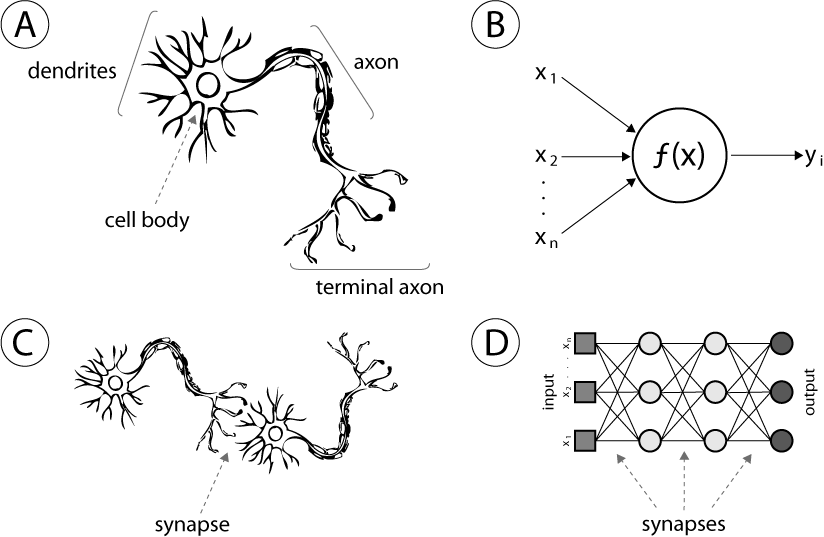
\includegraphics[scale=0.4]{ANN-NN}
	\caption{Unterschied zwischen einem ANN und einem NN \href{http://www.intechopen.com/source/html/39067/media/image1.png}{(source)}}
	\label{fig:ANN-NN}
\end{figure}
\noindent
Sie bieten eine alternative Möglichkeit zu den linearen Modellen der Datenverarbeitung. Die Neuronalen Netze modellieren
eine nicht lineare Beziehung zwischen Ein- und Ausgängen. Somit kann sich das Modell den Daten entsprechend anpassen,
egal wie die Daten verteilt sind. Es kann jede versteckte, mathematische Funktion zwischen den Daten und dem Ergebnis
erkennen und erlernen. Ein Problem der neuronalen Netze ist die enorme Menge an Rechenressourcen und Daten, die benötigt
werden, um gut zu funktionieren.
\newline
\newline
\textbf{Deep Neural Networks} ist eine weitere From von neuronalen Netzen. Der einzige Unterschied besteht darin, dass
\textit{deep neural network} mehrere hidden Layers haben und somit komplexere mathematische Zusammenhänge lernen
können. Diese Netzwerke kommen vor allem in der Bilderkennung zum Einsatz. Ein gutes Beispiel des Einsatzes eines
\textit{deep neural network} ist, die Erkennung von verschiedenen Gesichtern mittels einer Verkehrskamera. 
\newline
\newline
Einer der grössten Nachteile eines Neuronalen Netzes ist, dass es nicht weiss, welche Ereignisse vorher passiert sind.
Das heisst, es hat keine Erinnerungen an vergangene Handlungen. Im Bereich \gls{NLP} und \gls{NLG} ist dieser Nachteil
sehr bedeutsam, denn ohne sich an das vorher Geschehene zu erinnern, kann man keine Vorhersagen über zukünftige
Ereignisse treffen. Aus diesem Grund wurden spezielle neuronale Netze entwickelt, die eine Art von Gedächtnis haben, wie
zum Beispiel \gls{RNN} \ref{sub:rnn} oder LSTMs \ref{sub:lstm}, welche im nächsten Abschnitt genauer beschrieben werden.

\subsubsection{Prezeptron}
\label{sub:preceptron}
Künstliche neuronale Netze sind kein neues Konzept, anfänglich hiessen diese \flqq Prezeptronen\frqq \ und wurden
bereits um 1960 entwickelt. Diese Prezeptronen bestanden aus sogenannten McCulloch-Pitts-Neuronen. Diese wurden stetig
weiterentwickelt und es entstanden gewichtete, sowie mehrschichtige Prezeptronen, aus denen die heutigen künstlichen
neuronalen Netze entstanden.

\subsubsection{Aufbau}
\label{sub:structure-nn}
Neuronale Netze haben immer eine ähnliche Grundstruktur, sie bestehen aus sogenannten Schichten (\textit{eng.} Layers).
Diese Schichten sind einfache Gruppen von Neuronen, welche mittels Synapsen mit einer anderen Gruppe von Neuronen
verbunden sind. Die grundsätzliche Struktur eines \gls{ANN} beinhaltet eine Eingabeschicht (\textit{eng.} input layer),
mehrere versteckte Schichten (\textit{eng.} hidden layers) und eine Ausgabeschicht (\textit{eng.} output layer). In der
Eingabeschicht werden die Daten dem neuronalen Netz zur Verarbeitung gegeben. Die versteckten Schichten bestehen aus
mehreren Schichten von Neuronengruppen, welche die zu grundeliegende mathematische Funktion der Daten lernen. Am Schluss
hat jedes Netz noch eine Ausgabeschicht, wo die Resultate des Netzes ausgegeben werden. Dieser output layer hat immer
die Grösse des gewünschten Ergebnisses, d.h. wenn man ein \gls{NN} trainieren möchte um zwischen gesunden und
kranken Zellen zu unterscheiden, wird die Ausgabeschicht zwei Neuronen beinhalten.
\begin{figure}[H]
	\centering
	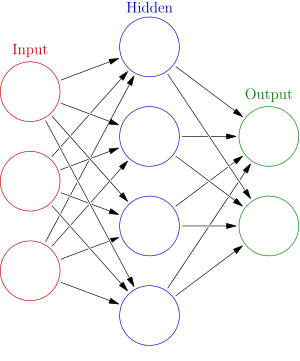
\includegraphics[scale=0.4]{NN_Structure}
	\caption{Struktur eines neuronalen Netzes \href{https://upload.wikimedia.org/wikipedia/commons/thumb/4/46/Colored_neural_network.svg/300px-Colored_neural_network.svg.png}{(source)}}
	\label{fig:NN-Structure}
\end{figure}

\subsubsection{Training}
\label{sub:training-nn}
Ein \gls{KNN} muss trainiert werden um die richtigen Berechnungen und die richtigen Gewichte in den
einzelnen Neuronen und Synapsen zu setzen. Dieses Training funktioniert im \textit{Supervised Learning} so, dass dem
\gls{KNN} eine vielzahl an Beispielen gegeben wird. Das neuronale Netz versucht dann, die gleichen Antworten wie im
Beispiel zu erhalten. Wenn es eine falsche Antwort voraussagt, wird ein Fehler berechnet und die Werte an jedem Neuron
und jeder Synapse werden für das nächste Mal rückwärts durch das \gls{NN} propagiert. Diesen Prozess nennt man
\textbf{Backpropogation} und wird in jedem \gls{KNN} verwendet, um die einzelnen Parameter anzupassen.

\subsubsection{Loss Funktion}
\label{sub:loss_fkt}
Das in \ref{sub:training-nn} beschriebene Training behilft sich einer sogenannten Loss Funktion um die Gewichte des
Netzes anzupassen. Dies ist eine Funktion um zu evaluieren, wie gut die aktuelle nichtlineare Funktion des \gls{KNN} die
Daten repräsentiert. Wenn die Vorhersagen des \gls{NN} weit von den echten Daten entfernt sind, gibt die Loss Funktion
einen hohen Wert aus. Wenn diese allerdings einigermassen ähnlich sind, ist der Wert der Funktion gering. 
\newline
\newline
Es wird zwischen Regression Loss und Classification Loss unterschieden. Regression Loss Funktionen
werden gebraucht bei Vorhersagen für kontinuierliche Werte. Classification Loss Funktionen werden gebraucht bei
Vorhersagen von kategorischen Labels, zum Beispiel ob es sich auf einem Bild um eine Katze oder einen Hund handelt.
\newline
\newline
Diese Funktion wird minimiert um ein möglichst gutes Ergebnis zu erhalten, dies geschieht mittels einem Optimizer
welcher in der Sektion \ref{sub:optimizer} genauer beschrieben wird.

\subsubsection{Optimizer}
\label{sub:optimizer}
Ein Optimizer im \gls{KNN} macht im Grunde nichts anderes als die \fullref{sub:loss_fkt} zu Optimieren indem diese
minimiert wird. Durch das kontinuierliche Minimieren der Loss Funktion performt das Modell nach jeder Iteration besser
und sucht die optimale Funktion um die Daten zu repräsentieren. Die Gewichte des \gls{NN} müssen nach jeder Iteration so
angepasst werden, dass die Loss Funktion, welche mittels dem Output berechnet wird, minimiert wird. Diese Anpassung kann
zum Beispiel mittels der Partiellen Ableitung der einzelnen Gewichte mit Respekt zum Loss berechnet werden. Dieser
spezielle Optimizer wird auch Gradient Descent genannt.

\section{Technische Konzepte}
\label{sec:technische-konzepte}
In diesem Abschnitt werden technische Konzepte genauer erklärt, welche in der Arbeit verwendet wurden. Diese Konzepte
sind meist sehr umfangreich und werden daher nur angeschnitten, so dass die weiteren Schlüsse dieser Arbeit
nachvollziehbar verstanden werden können.

\subsection{Markov Chains}
\label{sub:markov_chains}
Markov-Ketten gehören zu den frühesten Algorithmen im Bereich der Natural Language Generation. Sie sagen das nächste
Wort in einem Satz voraus, indem sie einfach das aktuelle Wort verwenden. Eine Markov-Kette berücksichtigt die Beziehung
zwischen jedem einzelnen Wort, um die Wahrscheinlichkeit des nächsten Wortes zu berechnen. Sie wurden in früheren
Versionen von Smartphone-Tastaturen verwendet, um Vorschläge für das nächste Wort im Satz zu generieren.
\newline
\newline
In Abbildung \ref{fig:markov-example} wird eine solche Kette anhand eines Beispiels von
\cite{andrew_adventure_markov_chain} dargestellt. Die Datensätze für die Markov Kette sind: \flqq I like turtles\frqq,
\flqq I like rabbits\frqq und \flqq I don't like snails\frqq. Die Abbildung \ref{fig:markov-example} bedeutet:
\begin{enumerate}
	\setlength\itemsep{0em}
	\item die Sätze zu 100\% mit einem \textit{I} starten
	\item gefolgt von einem \textit{like} zu 66\% und 33\% einem \textit{don't}
	\item das Wort \textit{don't} wird zu 100\% gefolgt von einem \textit{like}
	\item zum Schluss des Satzes gibt es zu 33\% entweder ein \textit{rabbits}, \textit{turtles} oder \textit{snails}
\end{enumerate}
\begin{figure}[H]
	\centering
	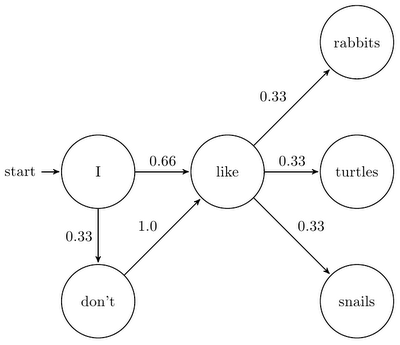
\includegraphics[scale=0.5]{markov_example}
	\caption{Visualisierung einer Markov Chain für Sequenzen}
	\label{fig:markov-example}
\end{figure}

\subsection{Recurrent Neural Networks}
\label{sub:rnn}
\gls{RNN} gehören zu den neusten Errungenschaften im Bereich der Neuronalen Netzen. Sie erlauben es, lange Sätze
zu verarbeiten mit einer deutlichen Verbesserung der Genauigkeit. \gls{RNN} ist eine spezielle Art der neuronalen
Netzwerke, welche sich die sequenzielle Natur der Eingabe zu nutzen macht. Jeder einzelne Teil der Sequenz (z.B. ein
Satz oder ein Vers) durchläuft ein Feedforward-Netzwerk und gibt die Ausgabe des Modells als Input für den nächsten Teil
der Sequenz, wie in Grafik \ref{fig:RNN-Overview} gut ersichtlich ist. Dies ermöglicht die Speicherung von Informationen aus
vorherigen Schritten, wie eine Art von Gedächtnis.
\newline
\newline
Durch dieses Gedächtnis über vorherige Schritte sind \gls{RNN} besonders beliebt bei Sprachgenerierung, da sie sich an den
Kontext des Satzes oder des Gespräches im Laufe der Zeit erinnern können. Aber nicht nur bei der Sprachgenerierung sind
\gls{RNN} beliebt, sondern auch bei: Spracherkennungen, Sprachmodellierungen und Übersetzungen.
\newline
\newline
\gls{RNN} haben einen grossen Nachteil, nämlich das Problem des verschwindenden Gradienten (\textit{eng.} \ \flqq
vanishing gradient problem\frqq). Mit zunehmender Länge der Sequenz verliert das Netzwerk die Erinnerung an Wörter die
weit zurück liegen und somit werden die Vorhersagen nur auf Grund von neuen Wörtern getroffen. Um dieses Problem zu
lösen wurden \gls{LSTM} \ref{sub:lstm} entwickelt, welche dieses Problem geschickt lösen.
\begin{figure}[H]
	\centering
	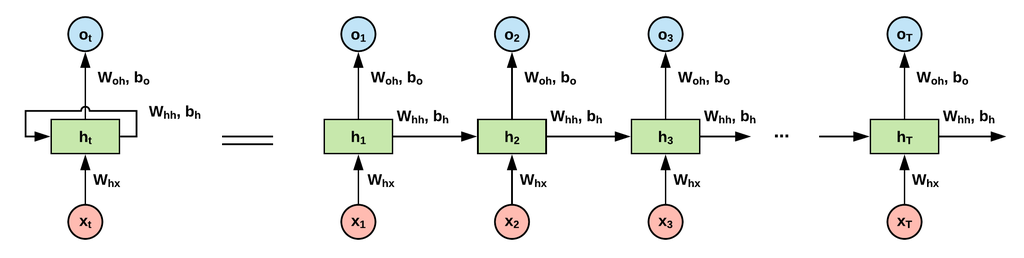
\includegraphics[scale=1.5]{RNN_Overview}
	\caption{Visualisierung eines RNN}
	\label{fig:RNN-Overview}
\end{figure}

\subsection{Long Short-Term Memory}
\label{sub:lstm}
\gls{LSTM} sind eine spezielle Art von Recurrent Neural Networks und somit auch eine Art von neuronalen Netzen. Die \gls{LSTM}
sind darauf ausgelegt, dass sie mit langen Sequenzen von Wörtern genauer arbeiten können. \gls{LSTM} unterscheiden sich von
herkömmlichen \gls{RNN} in einem wichtigen Punkt, nämlich haben die \gls{LSTM} ein vierschichtiges \gls{NN}. Normale
\gls{RNN} haben nur ein einschichtiges Netzwerk. Die kettenartige Struktur wurde auch in den \gls{LSTM}
gebraucht.
\newline
\newline
Das \gls{LSTM} hat die Fähigkeit, Informationen vom Zellzustand zu entfernen oder hinzuzufügen, welche sorgfältig durch
Strukturen reguliert werden, die als Gates bezeichnet werden. Gates sind eine Möglichkeit, Informationen optional
durchzulassen. Sie bestehen aus einer sigmoiden neuronalen Netzschicht und einer punktweisen Multiplikationsoperation,
wie in der Abbildung \ref{fig:LSTM-Gate} zu sehen ist. Die sigmoide Schicht des Netzwerks gibt eine Zahl zwischen Null
und Eins aus, welche beschreibt wie viel von dem Vektor durchgelassen werden soll. Ein Wert von Null bedeutet, dass
nichts durchgelassen werden soll und ein Wert von Eins bedeutet, dass alles durchgelassen werden soll. Ein \gls{LSTM}
hat drei solcher Gates um den Zellzustand zu kontrollieren.
\newline
\begin{figure}[H]
	\centering
	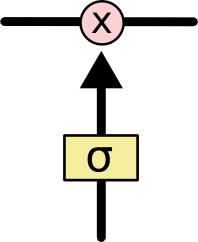
\includegraphics[scale=1]{LSTM_Gate}
	\caption{Visualisierung eines LSTM Gates \href{http://colah.github.io/posts/2015-08-Understanding-LSTMs}{(Colah's Blog)}}
	\label{fig:LSTM-Gate}
\end{figure}
\noindent
Ein Long Short-Term Memory besteht aus vier Komponenten, wie man der Grafik \ref{fig:LSTM-Overview} entnehmen kann:
\begin{enumerate}
	\setlength\itemsep{0em}
	\item einer Zelle (cell), beinhaltet den Zellzustand
	\item einem Eingangsgate (input gate)
	\item einem Ausgangsgate (output gate)
	\item einem Vergessensgate (forget gate)
\end{enumerate}
Diese Komponenten ermöglichen es dem Netzwerk, Wörter über beliebige Zeitintervalle zu merken oder diese auch wieder zu
vergessen, indem sie selber den Informationsfluss in und aus der Zelle regeln können. In der Zelle werden die
Informationen über vorgängige wichtige Wörter gespeichert, so dass auf diese zu einem späteren Zeitpunkt zugegriffen
werden können. Ausserdem kann das Netzwerk erkennen, wann ein Satzende eingetroffen ist und sich der Kontext ändert.
Durch diese Feststellung können durch das Vergessensgate Informationen übersprungen werden, welche in diesem Kontext für
nicht mehr relevant angeschaut werden. Dies ermöglicht es dem Netzwerk, selektiv nur relevante Informationen zu
verfolgen und gleichzeitig Informationen über einen längeren Zeitraum zu speichern.
\newline
\begin{figure}[H]
	\centering
	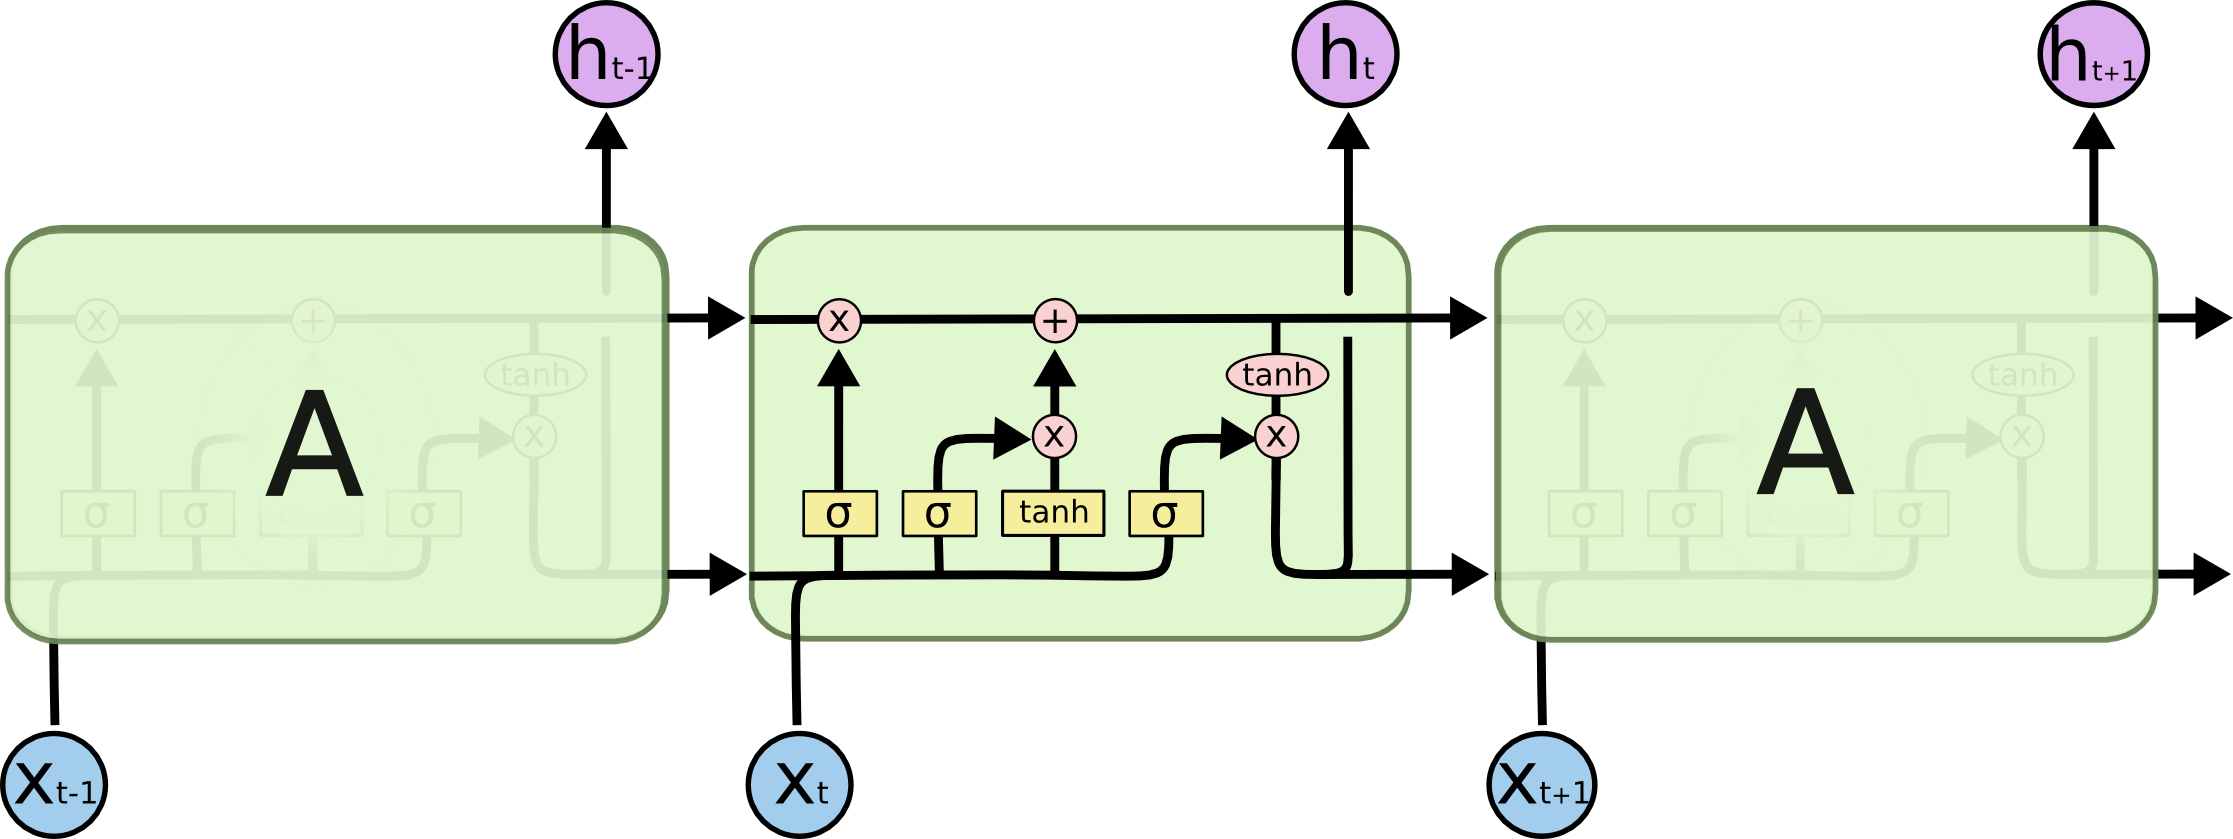
\includegraphics[scale=0.4]{LSTM_Overview_New}
	\caption{Visualisierung eines LSTM \href{http://colah.github.io/posts/2015-08-Understanding-LSTMs}{(Colah's Blog)}}
	\label{fig:LSTM-Overview}
\end{figure}
\noindent
\gls{LSTM} und ihre Variationen schienen die Antwort auf das \flqq vanishing gradient problem\frqq \ zu sein, jedoch gibt es
auch bei diesen Netzwerken gewisse Einschränkungen wie viele Informationen effektiv gespeichert werden können. Denn es
muss immer noch ein komplexer sequentieller Pfad der letzten Zelle zur nächsten Zelle übergeben werden. Dadurch
beschränkt sich die Länge der Sequenz, an die sich ein \gls{LSTM} noch erinnern kann, auf wenige hundert Wörter.
\newline
\newline
Ein weiterer Nachteil ist, dass \gls{LSTM} aufgrund ihrer hohen Rechenanforderungen sehr schwer zu trainieren sind. Aufgrund
ihrer sequentiellen Natur sind sie schwer zu parallelisieren und können somit den Vorteil der heutigen Rechengeräten wie
\gls{GPU} und \gls{TPU} nicht ausgiebig nutzen.

\subsubsection{Ablauf eines Schrittes im LSTM}
\label{sub:lstm-step-by-step}
\begin{figure}[H]
	\centering
	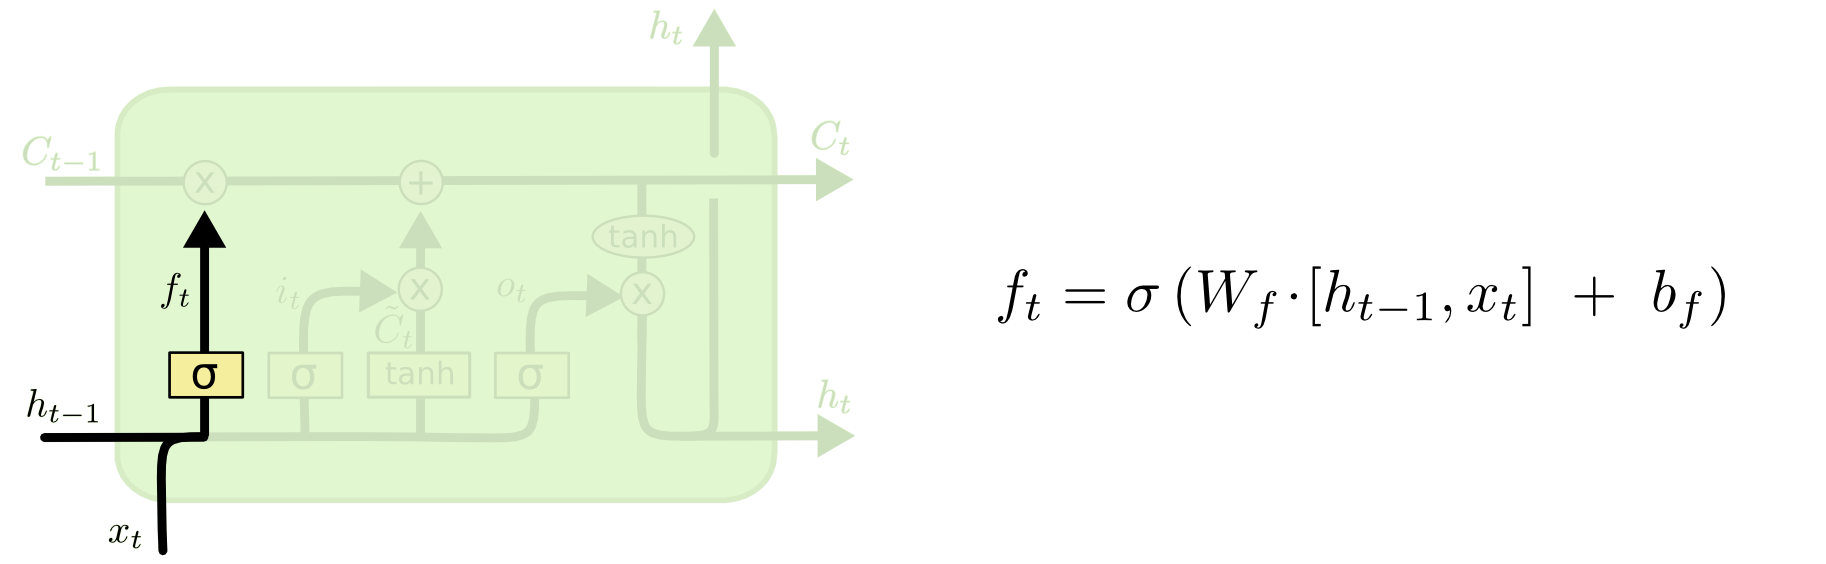
\includegraphics[scale=0.4]{LSTM_Forgetgate}
	\caption{Visualisierung eines LSTM Vergessensgates \href{http://colah.github.io/posts/2015-08-Understanding-LSTMs}{(Colah's Blog)}}
	\label{fig:LSTM-Forgetgate}
\end{figure}
\noindent
Der erste Schritt in einem \gls{LSTM} ist es zu entscheiden, welche Informationen aus der Zelle verworfen werden. Diese
Entscheidung wird durch die Sigmoid Funktion des Vergessensgates getroffen. Es schaut sich den Input $x_t$ und den
Output des vorherigen Wortes $h_{t-1}$ an und gibt eine Zahl zwischen $0$ bis $1$ aus für jeden einzelne Komponente des
Zellzustandvektor $C_{t-1}$. Eine $1$ bedeutet, dass der Wert komplett behalten werden soll. Eine $0$ hingegen bedeutet,
dass der Wert komplett verworfen werden soll. Dadurch entsteht ein \flqq Vergessensvektor\frqq \ $f_t$.
\newline
\begin{figure}[H]
	\centering
	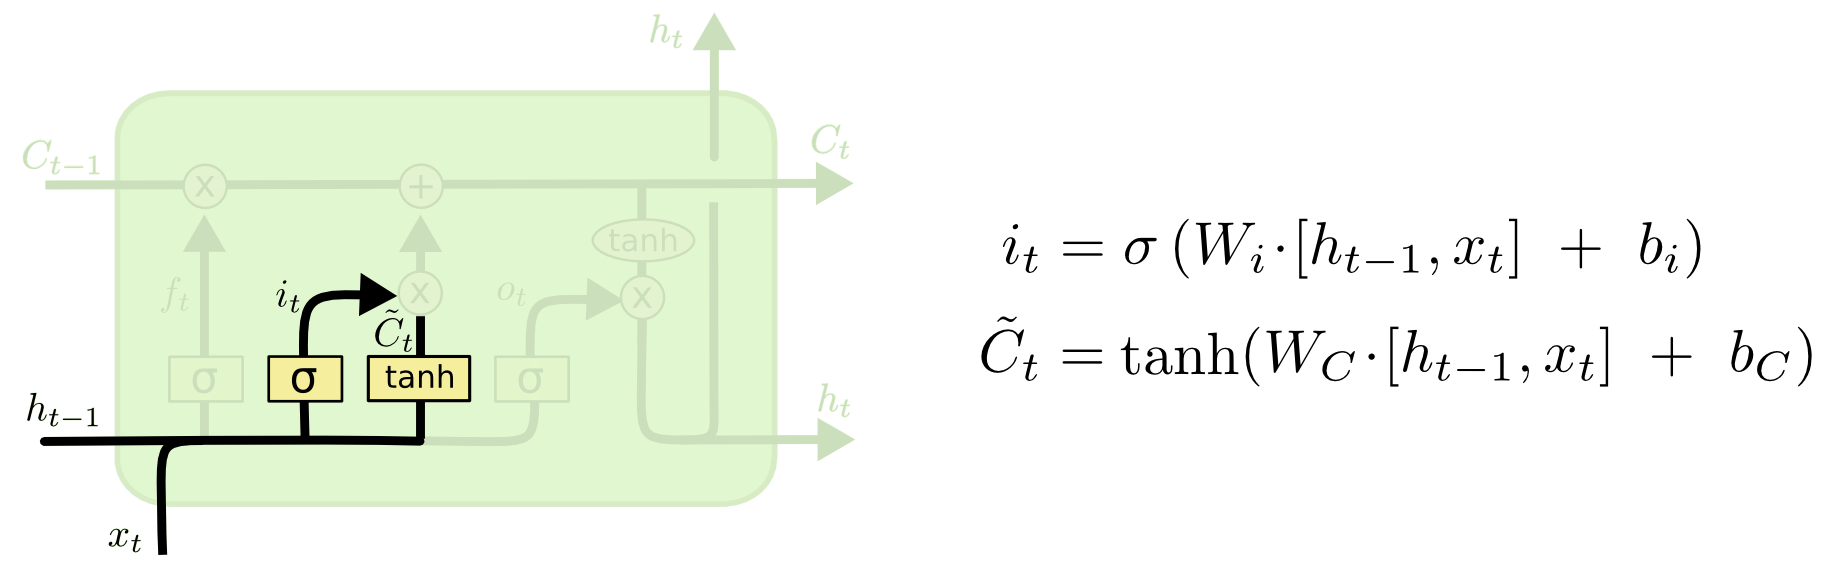
\includegraphics[scale=0.4]{LSTM_Inputgate}
	\caption{Visualisierung eines LSTM Eingangsgates \href{http://colah.github.io/posts/2015-08-Understanding-LSTMs}{(Colah's Blog)}}
	\label{fig:LSTM-Inputgate}
\end{figure}
\noindent
In einem nächsten Schritt wird darüber entschieden, welche neuen Informationen im Zellzustand gespeichert werden. Diese
Entscheidung wird in zwei Schritten getroffen. Als Erstes entscheidet die Sigmoid Funktion des Eingangsgates, welche
Werte aktualisiert werden und erstellt einen \flqq Aktualisierungsvektor\frqq \ $i_t$, welcher für jeden Wert des
Zellzustands eine Zahl zwischen $0$ und $1$ beinhaltet. Als nächstes erstellt eine Tanh Funktion einen neuen
Zellzustandvektor $\tilde{C}_t$ mit den aktualisierten Werten des Zustands. In einem nächsten Schritt werden die beiden
Vektoren $i_t$ und $\tilde{C}_t$ kombiniert und der Zellzustand wird aktualisiert.
\newline
\newline
Anschliessend wird der alte Zellzustand $C_{t-1}$ zum neuen Zustand $C_t$ aktualisiert. Der alte Zustand wird mit dem
berechneten \flqq Vergessensvektor\frqq \ $f_t$ multipliziert, um die Dinge zu vergessen, die irrelevant geworden sind.
Dann multiplizieren wir das Ergebnis des vorherigen Schrittes mit dem \flqq Aktualisierungsvektor\frqq \ $i_t$
kombiniert mit dem neuen Zellzustandvektor $\tilde{C}_t$. Aus dem ergibt sich der neue Zellzustand $C_t$.
\newline
\begin{figure}[H]
	\centering
	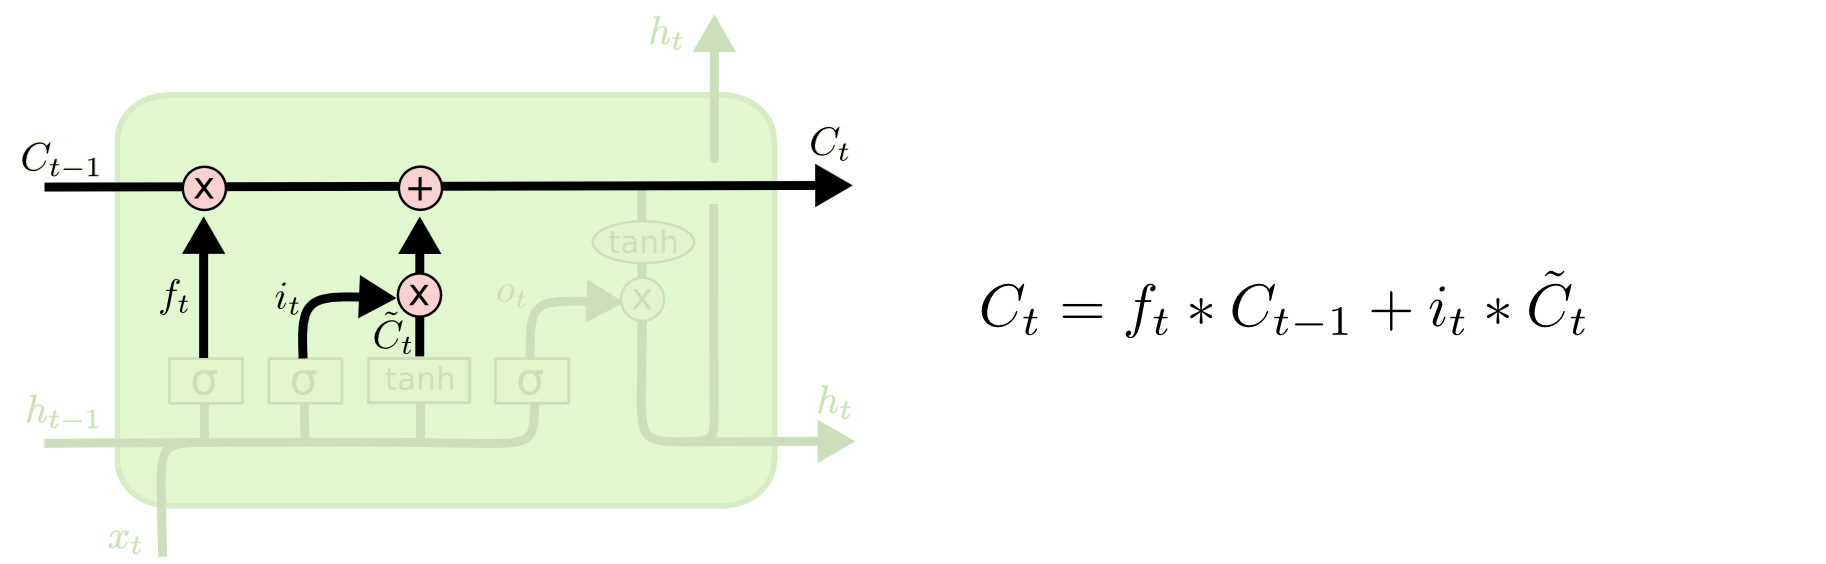
\includegraphics[scale=0.4]{LSTM_Addition}
	\caption{Visualisierung der Addition der Vektoren eines LSTMs \href{http://colah.github.io/posts/2015-08-Understanding-LSTMs}{(Colah's Blog)}}
	\label{fig:LSTM-Addition}
\end{figure}
\noindent
Schliesslich muss entschieden werden, was ausgegeben werden soll, diese Entscheidung wird im Ausgangsgate getroffen. Der
Output basiert auf dem neuen Zellzustandvektor $C_t$, wird aber vorgängig noch gefiltert. Zuerst wird eine Sigmoid
Funktion auf dem Input $x_t$ und dem Output des vorherigen Wortes $h_{t-1}$ ausgeführt, um zu entscheiden welche Teile
des Zustandes ausgegeben werden. Dann wird der aktuelle Zellzustand $C_t$ mittels einer Tanh Funktion auf die Werte
zwischen $-1$ und $1$ gebracht und anschliessend mit dem Resultat der Sigmoid Funktion multipliziert. Somit werden nur
die Teile ausgegeben, die wirklich relevant sind.
\newline
\begin{figure}[H]
	\centering
	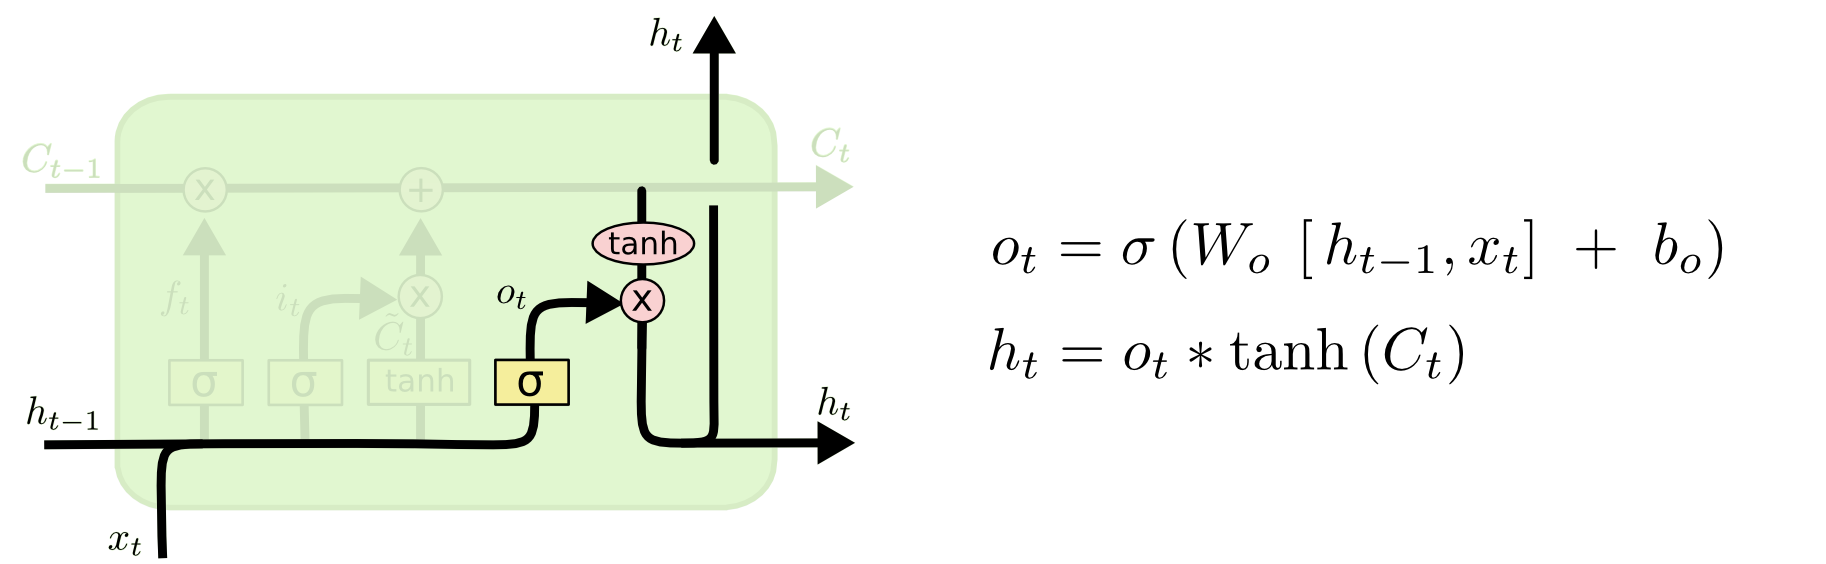
\includegraphics[scale=0.4]{LSTM_Outputgate}
	\caption{Visualisierung eines LSTM Ausgangsgate \href{http://colah.github.io/posts/2015-08-Understanding-LSTMs}{(Colah's Blog)}}
	\label{fig:LSTM-Outputgate}
\end{figure}

\subsection{Autoencoder}
\label{sub:autoencoder}
Autoencoder sind eine spezielle Art von \gls{KNN}, welche oft verwendet werden, um effiziente
Datencodierungen auf unbeaufsichtigte (unsupervised) Weise zu erlernen. Ein Autoencoder besteht auf der einen Seite aus
einem Encoder und auf der anderen aus einem Decoder. 
\newline
\newline
Das Ziel des Encoders ist es, eine Darstellung für einen Datensatz zu erlernen, typischerweise mit dem Zweck der
Reduzierung der Dimensionalität. Indem das Netzwerk trainiert wird, lernt es das Rauschen oder Unreinheiten zu
ignorieren und sich auf die echten Daten zu konzentrieren.
\newline
\newline
Der Decoder hat das Ziel, aus der reduzierten Codierung eine Darstellung zu rekonstruieren, die seiner ursprünglichen
Form so nahe wie möglich kommt.
\newline
\newline
Durch diese Eigenschaft der Komprimierung und der Rekonstruktion werden Autoencoder effektiv zur Lösung vieler Probleme
eingesetzt, von der Gesichtserkennung bis zum Erlangen der semantischen Bedeutung für die Worte.
\begin{figure}[H]
	\centering
	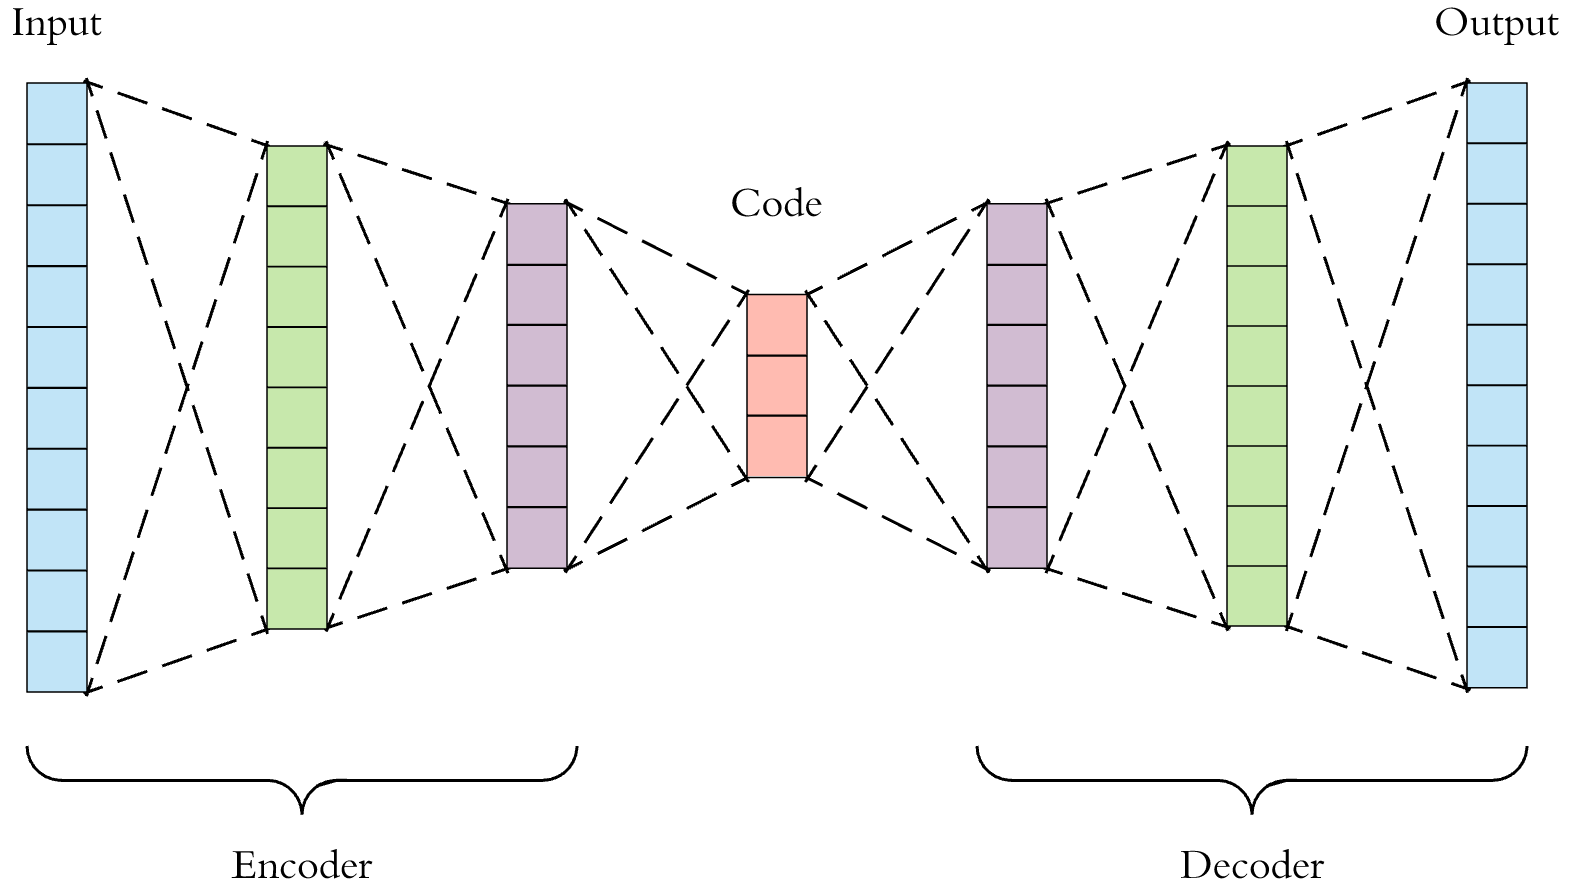
\includegraphics[scale=0.2]{autoencoder}
	\caption{Visualisierung eines Autoencoders}
	\label{fig:Autoencoder}
\end{figure}

\subsection{Transformer}
\label{sub:transformer}
Transformer sind eine weitere Art von \gls{KNN}, welche sehr intuitiv verstanden werden können. Die
Hauptaufgabe besteht darin, einen Input (z.B. einen deutschen Satz) in einen Output (z.B. in einen englischen Satz) zu
transformieren. Das Transformermodell besteht aus mehreren Encoder- und Decoder Komponenten, welche zusammen verbunden
sind. Die Encoder Komponenten sind nichts weiteres als mehrere Encoders, welche aufeinander gestapelt werden und eine
Verbindung zum oberen Encoder haben. Dasselbe wird auch bei der Decoder Komponente gemacht, dort werden mehrere
Decoders aufeinander gestapelt und sind mit dem oberen Layer verbunden. Der oberste Encoder der Encoder Komponente ist
mit jedem Decoder der Decoder Komponente verbunden. Dem ersten Encoder wird der Input übergeben und der letzte Decoder
liefert den gewünschten Output.
\newline
\newline
Transformatoren wurden entwickelt, um das Problem der Sequenztransduktion (Transformation einer Eingangssequenz zu einer
Ausgangssequenz) oder der neuronalen maschinellen Übersetzung zu lösen. Dazu gehören Spracherkennung, Text-zu-Sprache
Transformation, Übersetzungen und noch viele weitere.
\begin{figure}[H]
	\centering
	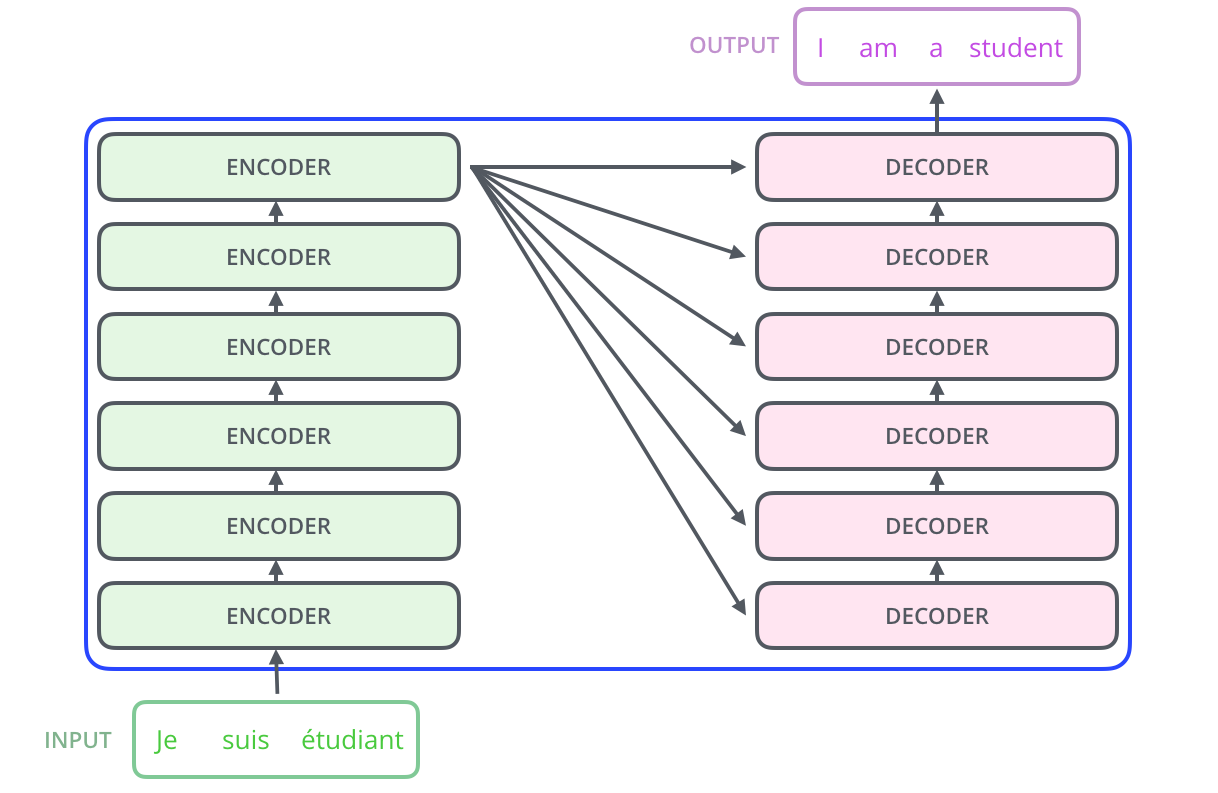
\includegraphics[scale=0.3]{transformer}
	\caption{Visualisierung eines Transformers}
	\label{fig:Transformer}
\end{figure}

\subsection{Generative Adversarial Networks}
\label{sub:gan}
\gls{GAN} verfolgen einen spieltheoretischen Ansatz, im Gegensatz zu einem herkömmlichen
neuronalen Netzwerk. Das Netzwerk erlernt die Generierung aus einer Trainingsverteilung durch ein 2-Spieler-Spiel. Die
beiden Spieler sind der Generator und der Diskriminator. Diese beiden Gegner befinden sich während des gesamten
Trainingsprozesses im ständigen Kampf miteinader. Da eine gegensätzliche (adversielle) Lernmethode angewandt wird,
beinhaltet das Netzwerk einige Eigenheiten.
\newline
\newline
Der Generator wird verwendet um aus einem zufälligen Rauschen möglichst echte Daten zu generieren. Und der Diskriminator
hingegen soll unterscheiden können, ob es sich bei den Daten um echte oder generierte Daten handelt. Die beiden Instanzen
befinden sich im konstanten Kampf gegeneinader, wobei der Generator, versucht möglichst echte Daten zu erzeugen und der
Diskriminator versucht sich nicht täuschen zu lassen. Um möglichst echte Daten zu generieren, benötigt es einen sehr
guten Generator, so wie einen sehr guten Diskriminator. Dies liegt daran, dass wenn der Generator nicht gut genug ist, er
nie in der Lage sein wird, den Diskriminator zu täuschen und das Modell nie konvergieren wird. Wenn aber der
Diskriminator schlecht ist, dann werden auch Bilder, welche keinen Sinn geben, als echt eingestuft. Dadurch kann das
Modell nicht korrekt trainiert werden, denn es gibt keinen genug guten \flqq Validator\frqq \ der Daten.
\newline
\newline
Der Ablauf eines Schrittes in einem \gls{GAN} fängt mit der Erzeugung eines Zufallsrauschens an. Dieses Rauschen wird danach
dem Generator übergegeben, welcher daraus einen möglichst echten Datensatz generiert. Dieser generierte Datensatz wird
anschliessend dem Diskriminator übergeben, welcher entscheidet ob die Daten generiert oder echt sind und gibt demnach
ein entsprechendes Label aus.
\begin{figure}[H]
	\centering
	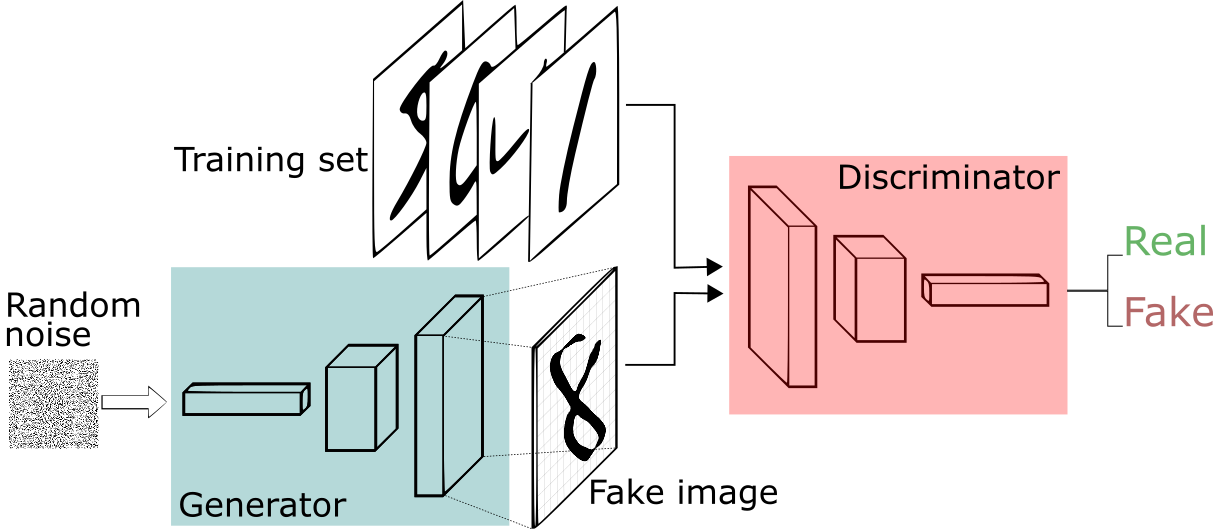
\includegraphics[scale=0.3]{gan}
	\caption{Visualisierung eines GANs}
	\label{fig:GAN}
\end{figure}

\subsection{Aktivierungsfunktionen}
\label{sub:activation-functions}
Aktivierungsfunktionen werden in \gls{NN} gebraucht, um die Ausgaben der einzelnen Layers zu bestimmen. Die
Ausgaben der Layers können mit Ja oder Nein verglichen werden, nur sind es bei den Aktivierungsfunktionen entweder eine
$0$ bis $1$ oder $-1$ bis $1$, je nach Funktion. Aktivierungsfunktionen lassen sich in zwei Typen unterteilen: lineare
Aktivierungsfunktionen und nicht lineare Aktivierungsfunktionen.

\subsubsection{Lineare Aktivierungsfunktionen}
\label{sub:linear-activation}
\begin{figure}[H]
	\centering
	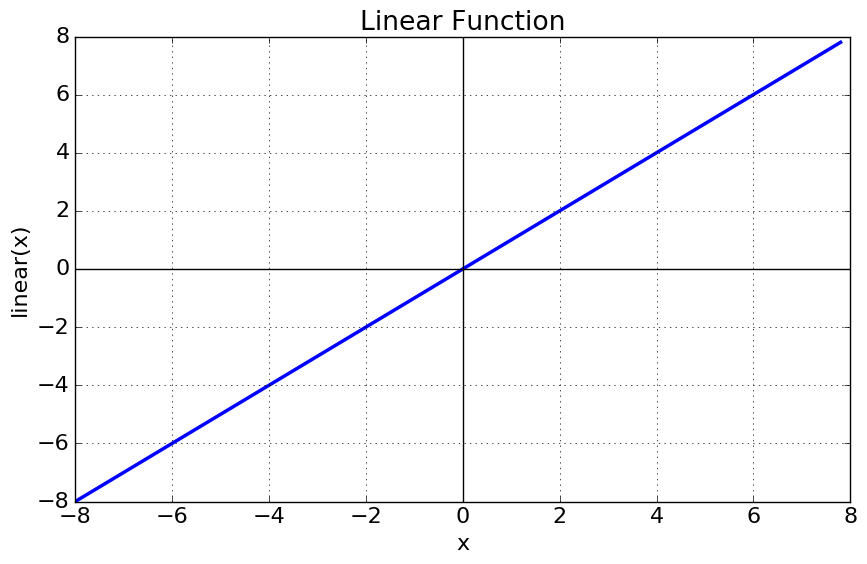
\includegraphics[width=7cm]{Linear_Activation}
	\caption{Lineare Aktivierungsfunktion}
	\label{fig:Linear-Activation}
\end{figure}
\noindent
Bei der linearen Aktivierungsfunktion ist die Funktion eine Linie, die stetig steigt. Daher ist die Ausgabe der Funktion
nicht auf einen Bereich beschränkt. Eine solche Funktion kann zum Beispiel $f(x) = x$ sein, diese befindet sich im
Bereich von $-\infty \ \text{bis} \ \infty$. Das Problem bei linearen Funktionen ist, dass die Daten meist nicht linear
verteilt sind und somit kann sich das Modell nicht genügend den Daten anpassen.

\subsubsection{Nicht lineare Aktivierungsfunktionen}
\label{sub:nonlinear-activation}
\begin{figure}[H]
	\centering
	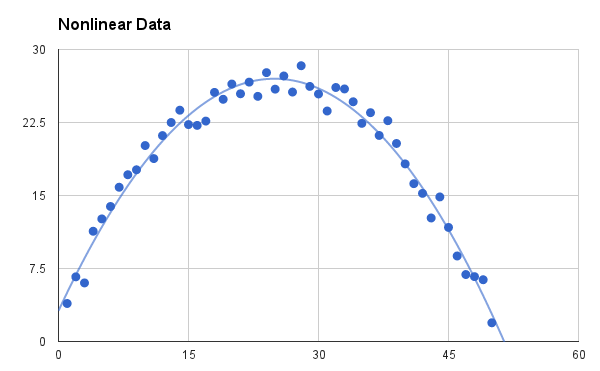
\includegraphics[width=7cm]{Nonlinear_Activation}
	\caption{Nicht lineare Aktivierungsfunktion}
	\label{fig:Nonlinear-Activation}
\end{figure}
\noindent
Nicht lineare Aktivierungsfunktionen werden für die Ausgabe von Layern der neuronalen Netzen am häufigsten verwendet.
Durch die nicht Linearität kann sich das Modell leicht, verschiedensten verteilten Daten anpassen und sehr viele
verschiedene \flqq Formen\frqq annehmen. Eine solche Funktion kann zum Beispiel $f(x) = x^2$ sein.

\subsubsection{Sigmoid}
\label{sub:activation-sigmoid}
\begin{figure}[H]
	\centering
	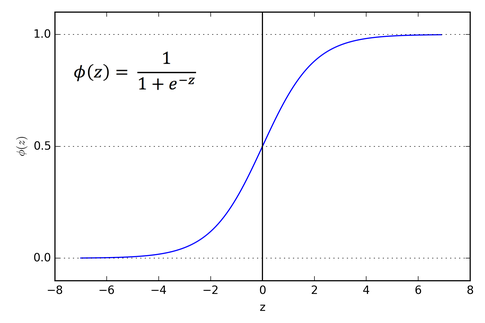
\includegraphics[width=7cm]{Activation_Sigmoid}
	\caption{Sigmoid Funktion}
	\label{fig:Activation-Sigmoid}
\end{figure}
\noindent
Eine Sigmoidfunktion ist eine mathematische Funktion mit einem S-förmigen Graphen, sie ist eine der weitverbreitesten
Funktionen im Umgang mit neuronalen Netzen. Der Grund dafür ist, dass sie sich zwischen $0$ und $1$ befindet. Dadurch
ist die Sigmoidfunktion sehr nützlich an Orten, wo man eine Vorhersage über Wahrscheinlichkeiten treffen muss, da sich
Wahrscheinlichkeiten auch immer zwischen $0$ und $1$ befinden.
\newline
Ein Problem der Sigmoidfunktion ist, dass Parameter \flqq stecken bleiben\frqq \ können, weil sich der Bereich der
Funktion nur zwischen $0$ und $1$ befindet. Somit ist es möglich, dass Parameter die sich sehr nahe bei $0$ befinden nur
wenig angepasst werden und somit gleich bleiben. Dies kann bei Parametern passieren, welche erst nach einer gewissen
Zeit zum Vorschein kommen.

\subsubsection{Tanh}
\label{sub:activation-tanh}
\begin{figure}[H]
	\centering
	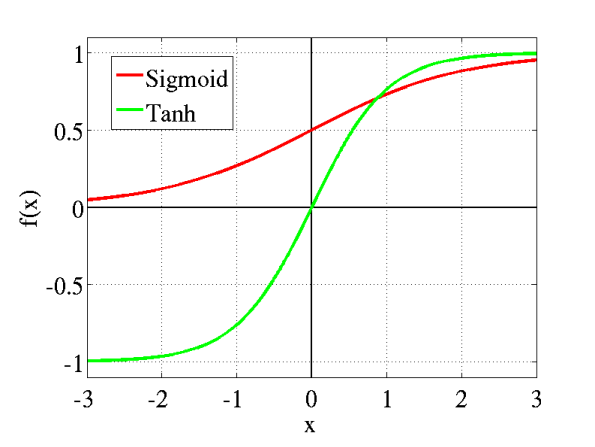
\includegraphics[width=7cm]{Activation_Tanh}
	\caption{Tanh Funktion}
	\label{fig:Activation-Tanh}
\end{figure}
\noindent
Wie die Sigmoidfunktion, ist auch die Tanhfunktion eine mathematische Funktion mit einem S-förmigen Graphen, gibt aber
stattdessen Werte im Bereich von $-1$ und $1$ aus. Somit können stark negative Einträge in der Funktion negativ
abgebildet werden, was in der Sigmoidfunktion nicht möglich ist. Zusätzlich werden nur $0$ ähnliche Einträge auf nahezu
$0$ abgebildet, somit wird das \flqq stecken bleiben\frqq \ beim Training eines Parameters unwahrscheinlicher.
\newline
Die Tanhfunktion wird vor allem bei der Klassifikation von zwei verschiedenen Klassen verwendet.

\subsubsection{ReLU (Rectified Linear Unit)}
\label{sub:activation-relu}
\begin{figure}[H]
	\centering
	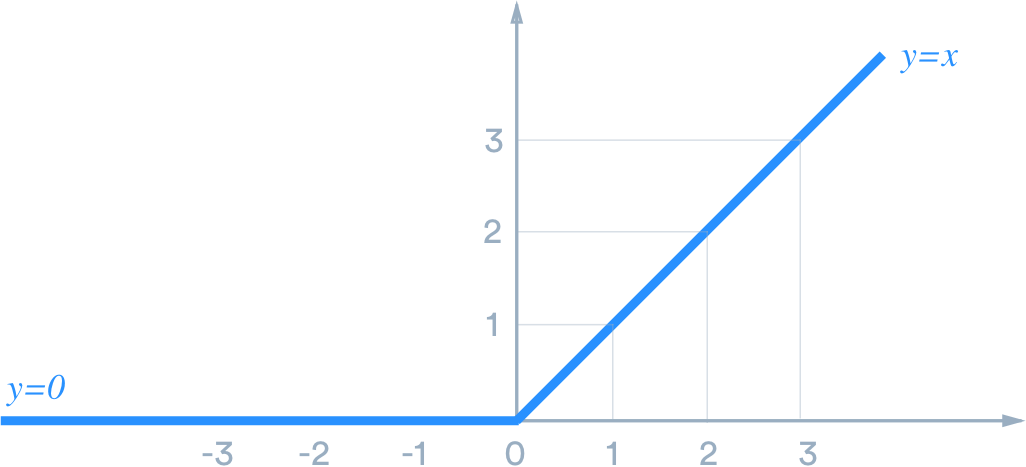
\includegraphics[width=7cm]{Activation_ReLU}
	\caption{ReLU Funktion}
	\label{fig:Activation-Relu}
\end{figure}
\noindent
ReLU ist die am weitesten verbreitete und die am meisten benutzte Aktivierungsfunktion. Sie wird vor allem in
Convolutional Neural Networks sowie in den meisten Deep Learning Modellen gebraucht. Der Bereich der Funktion ist von $0
\ \text{bis} \ \infty$. Ausserdem ist die Funktion, sowie ihre Ableitung monoton.
\newline
Das Problem der ReLU Aktivierungsfunktion ist das Abbilden der negativen Werte, denn jede negative Eingabe der Funktion
wird zu $0$ werden. Dies verringert die Fähigkeit des Modells sich den Daten richtig anzupassen und zu trainieren, denn
die negativen Werte können nicht entsprechend abgebildet werden. Aus diesem Grund wurde die \textbf{Leaky ReLU
Aktivierungsfunktion} entwickelt, welche dieses Problem löst.

\subsection{N-Gramm}
\label{sub:n-gramm}
N-Gramme sind das Ergebnis der Zerlegung eines Textes oder Satzes in einzelne Fragmente. Der Text wird dabei zerlegt und
jeweils $N$ aufeinanderfolgende Fragmente werden als N-Gramme zusammengefasst. Die Fragmente können Buchstaben, Wörter
oder ähnliches sein. Die Zerlegung eines Satzes in N-Gramme wird vor allem zur Hilfe von Analysen oder statistischen
Auswertungen gebraucht.
\newline
Es gibt verschiedene Arten von N-Grammen. Wichtige Arten sind zum Beispiel Monogramme, bei dem $N = 1$, oder Bigramme,
bei dem $N = 2$ ist. Wobei $N$ für die Anzahl Zeichen steht die betrachtet werden.
\newline
\newline
\textbf{Beispiel:}
\begin{align*}
	s (\text{Zeichenkette}) &= \text{\glqq WIPRO\grqq} \\
	N (\text{Anzahl Zeichen}) &= 2\ (\text{Bigramm}) \\
	f (\text{Frequenzwektor}) &= \{\_W:1, WI:1, IP:1, PR:1, RO:1, O\_:1\}
\end{align*}

\subsection{Metriken}
\label{sub:metrics}
Im Bereich von \gls{NLG} sind Metriken ein zentales Thema, da dort ein Vergleich von Labels nicht reicht. Daher mussten
neue Metriken entwickelt werden, die auf den Inhalt der Eingabe und Ausgabe Daten schauen und auf Grund dieses einen
Wertes berechnen wie gut die beiden Daten zusammenpassen. Diese Problematik ist komplex, denn es gibt keinen Blueprint,
der für jeden Fall passt. Eher gibt es einen ganzen Stapel an verschiedenen Methoden zur Auswertung, aus denen eine
entsprechende Metrik gewählt werden muss.
\newline
\newline
Die Intuition für die Bewertung von generiertem Text ist die gleiche wie für die Bewertung von Labels. Wenn der Text $A$
näher an einem der Referenztexte liegt als der Text $B$, dann soll $A$ höher bewertet werden als $B$. Wie bei anderen
Verfahren basiert diese Übereinstimmung auf Präzision (Spezifität, \textit{eng.} specifity) und Erinnerung
(Sensitivität, \textit{eng.} sensitivity). Einfach ausgedrückt, $A$ ist genauer als $B$, falls der Prozentsatz von $A$,
der mit einem Referenztext übereinstimmt, höher ist als $B$. Die Erinnerung von $A$ ist höher, wenn er mehr
übereinstimmenden Text aus einer Referenz enthält als $B$.

\subsubsection{\gls{BLEU}}
\label{sub:BLEU}
\gls{BLEU} ist die weitverbreiteste Metrik für die Bewertung von maschinellen Übersetzungssystemen. Sie wurde im Juli
2002 von einer Forschungsgruppe von IBM entwickelt, da bis dort hin die Metriken zur Auswertung von Machine Translation
zu ineffizient waren. Die Grundsatz Idee von \gls{BLEU} ist: \gls{BLEU} Scores sollen den Unterschied zwischen
Referenzübersetzungen und maschinellen Übersetzungen messen. Dafür werden Präzision und Erinnerung durch modifizierte
n-Gramm-Präzision bzw. beste Abgleichlänge approximiert. 
\newline
\newline
Zunächst werden einzelne Segmente (meist Sätze) verglichen, später wird ein Durchschnittswert für den gesamten Text
ermittelt. Je näher die maschinelle Übersetzung der Referenzübersetzungen kommt, umso besser ist ihr Score. Generell wird
dabei eine Skala von $0$ bis $1$ verwendet, auf welcher der Wert $1$ identisch mit der qualitativ hochwertigen
Referenz-Übersetzung ist, während ein Score von $0$ signalisiert, dass die maschinelle Übersetzung keine
Übereinstimmungen mit der Referenz hat.
\newline
\newline
Ein \gls{BLEU} Score von $1$ ist nicht erstrebenswert, denn dies würde bedeuten, dass die maschinelle Übersetzung
identisch mit der Referenz ist. Dies sollte jedoch in keinem Fall das Ziel sein. Es sollte versucht werden, eine
möglichst korrekte Übersetzung zu liefern und nicht die Referenzübersetzungen zu imitieren.

\paragraph{Interpretation} Es wird dringend davon abgeraten, BLEU-Werte über verschiedene Korpusse und Sprachen hinweg
zu vergleichen. Auch der Vergleich der BLEU-Werte für denselben Korpus, aber mit einer abweichenden Anzahl von
Referenzübersetzungen, kann sehr irreführend sein. Die genauere Interpretation des Wertes ist in Tabelle
\ref{tab:BLEU-Interpretation} ersichtlich.

\begin{table}[ht]
	\begin{tabular}{| c | l |}
	\hline
	BLEU-Wert            & Interpretation                                                            \\ \hline
	\textless \ 0.1      & Fast unbrauchbar                                                          \\
	0.1 – 0.2            & Schwierig, das Wesentliche zu verstehen                                   \\
	0.2 – 0.3            & Das Wesentliche ist verständlich, aber es gibt erhebliche Grammatikfehler \\
	0.3 – 0.4            & Verständliche bis gute Übersetzungen                                      \\
	0.4 – 0.5            & Hochwertige Übersetzungen                                                 \\
	0.5 – 0.6            & Sehr hochwertige, adäquate und flüssige Übersetzungen                     \\
	\textgreater \ 0.6   & Qualität oft besser als menschliche Übersetzungen 					     \\
	\hline                        
	\end{tabular}
	\caption{Interpretation des BLEU Wertes}
	\label{tab:BLEU-Interpretation}
\end{table}

\paragraph{Mathematischen Details}
Mathematisch wird der BLEU-Score definiert mit ~\autocite{modelle_bewerten_bleu}:

\begin{equation}
	\text{BLEU} = \underbrace{\vphantom{\prod_i^4}\min\Big(1,\exp\big(1-\frac{\text{reference-length}}{\text{output-length}}\big)\Big)}_{\text{brevity penalty}}
\underbrace{\Big(\prod_{n=1}^{4}
\text{precision}_n\Big)^{1/4}}_{\text{n-gram overlap}}
\end{equation}
\myequations{BLEU Score}
mit
\begin{equation}
	\text{precision}_n = \dfrac{\sum_{\text{sentence}\in\text{Candidates-Corpus}}\sum_{n\in\text{sentence}}\min(m^n_{cand}, m^n_{ref})}
{w_t^n = \sum_{\text{sentence'}\in\text{Candidates-Corpus}}\sum_{n'\in\text{sentence'}} m^{n'}_{cand}}
\end{equation}
\myequations{Precision im BLEU Score}
wobei $n$ die Anzahl an \textit{n-grams} ist.
\newline
\newline
Wobei Folgendes gilt:
\begin{itemize}
	\setlength\itemsep{0em}
	\item $m^n_{cand}$ entspricht der Anzahl an n-Gramme für den Kandidaten, die mit der Referenzübersetzung
	übereinstimmen
	\item $m^n_{ref}$ entspricht der Anzahl an n-Gramme in der Referenzübersetzung
	\item $w^i_t$ entspricht der Gesamtzahl der n-Gramme in der Kandidatenübersetzung
\end{itemize}
Die Formel besteht aus zwei Teilen: dem Abzug für die Kürze (\textit{eng.} brevity penalty) und der N-Gramm
Übereinstimmung (\textit{eng.} n-gram overlap).
\begin{itemize}
	\setlength\itemsep{0em}
	\item Der Abzug für die Kürze bestraft generierte Übersetzungen, die verglichen mit der ähnlichsten Referenzlänge
	exponentiell abnehmend zu kurz sind. Dies kompensiert den fehlenden Trefferquoten (\textit{eng.} recall) Term.
	\item Die N-Gramm-Übereinstimmung zählt, wie viele N-Gramme mit ihrem N-Gramm-Gegenstück in den
	Referenzübersetzungen übereinstimmen. Über die N-Gramm-Übereinstimmung wird die Genauigkeit (\textit{eng.}
	precision) der Übersetzung gemessen. Kürzere N-Gramme ermitteln die Ädequatheit, längere N-Gramme die Flüssigkeit
	der Übersetzung. Zur Vermeidung einer unnötigen Zählung wird die N-Gramm-Zählung auf die maximale N-Gramm-Anzahl
	begrenzt, die in der Referenz auftritt ($m_{ref}^n$).
\end{itemize}

\subsubsection{\gls{TER}}
\label{sub:TER}
Während es bei \gls{BLEU} vor allem darum geht, zu bestimmen, wie nah eine maschinelle Übersetzung einer Referenz kommt,
sagt \gls{TER} aus, wie viele Schritte im Post-Editing benötigt werden, um von der erstellten maschinellen Übersetzung
zur korrekten Übersetzung zu gelangen. \gls{BLEU} und \gls{TER} sind sich in vielerlei Hinsicht sehr ähnlich und werden
daher gerne zusammen verwendet.
\newline
\gls{TER} wie auch \gls{BLEU}, interessieren sich nicht für die zu grunde liegende Sprache des Satzes, sonden der
Algorithmus möchte nur herausfinden, wie viele Unterschiede es zwischen dem Referenzsatz und dem generierten Satz gibt.
\newline
Auch \gls{TER} benötigt einen Referenzkorpus an dem gemessen werden soll, wie nahe der generierte Output der Referenz
kommt.
\newline
Diese Metrik wird dazu verwendet um zu prüfen, wie viele verändernde Schritte nötig sind um ein gutes Ergebnis zu
erhalten.
\begin{equation}
	\text{TER} = \frac{\text{\# of edits}}{\text{average \# of references}}
\end{equation}
\myequations{TER Score}

\section{Stand im Bezug auf eigenes Projekt}
\label{sec:stand-bezug-projekt}
Alle erwähnten technischen Konzepte sind längst keine eigenständigen, geschlossenen Einheiten mehr. Sondern werden in
den aktuellen Forschungen miteinader verknüpft und es werden vielversprechende Ansätze von einem Konzept ins Andere
übernommen, um neue Architekturen für verschiedene Probleme zu entwickeln. Auf diese Art und Weise sind die meisten
Durchbrüche der aktuellen Forschung gelungen.
\newline
\newline
Eines der aktuellsten Themen im Bereich von \fullref{sub:natural-language-generation} und
\fullref{sub:natural-language-processing} ist \fullref{sub:neural-style-transfer}, welches in momentanen Forschungen auf
Textbasierte Daten angewendet wird, mit moderaten Ergebnissen, um den Stil eines Satzes auf einen anderen zu übertragen.
Bei diesem Ansatz werden meist \fullref{sub:rnn}, \fullref{sub:lstm}, \fullref{sub:autoencoder} und viele weiter der
oben erwähnten Konzepte verwendet.
